\chapter{Fundamentação Teórica}
\label{chap:fundteor}

\begin{flushright}

   \begin{list}{}{
      \setlength{\leftmargin}{4.5cm}
      \setlength{\rightmargin}{0cm}
      \setlength{\labelwidth}{0pt}
      \setlength{\labelsep}{\leftmargin}}
      \item Quanto maior for a rapidez de transformação de uma
      sociedade, mais temporárias são as necessidades
      individuais. Essas flutuaçõess tornam ainda mais acelerado
      o senso de turbilh da sociedade.

      \begin{list}{}{
      \setlength{\leftmargin}{0cm}
      \setlength{\rightmargin}{0cm}
      \setlength{\labelwidth}{0pt}
      \setlength{\labelsep}{\leftmargin}}
      \item (Alvin Toffler)
      \end{list}
   \end{list}
\end{flushright}

\begin{flushright}
  Quanto maior for a rapidez de transformação de uma \\
  sociedade, mais temporárias são as necessidades \\
  individuais. Essas flutuações tornam ainda mais \\
  acelerado o senso de turbilhão da sociedade. \\
  \ \\
  (Alvin Toffler)
\end{flushright}

%--------- NEW SECTION ----------------------
\section{Ultra Wide Band}
\label{sec:sota}
O princípio de funcionamento do Pozyx se dá na utilização da tecnologia 
de Ultra Wide Band (UWB) ou de banda ultra larga. UWB é um protocolo de comunicação sem fio
assim como o Wi-fi e o Bluetooth. Contudo, seu funcionamento difere um pouco destas e outras tecnologias,
trazendo vantagens e desvantagens. O uso e os estudos acerca da tecnologia UWB vêm se desenvolvendo
há cerca de 100 anos, quando o inventor e físico italiano Guglielmo Marconi (1874-1937), baseando-se na teoria 
de Maxwell sobre ondas eletromagnéticas, estudava os princípios da transmissão de dados por radiofrequência. Futuramente 
foi utilizada em radares do exército estado-unidense e, entre os anos de 1960 a 1990 ficou restrita aplicações militares.

%--------- NEW SECTION ----------------------
\section{Características da tecnologia}
\label{sec:ass1}
Como mencionado anteriormente, a tecnologia UWB possui algumas diferenças de funcionamento,
quando comparada a outras de comunicação \textit{Wireless}. 

\subsection{Vantagens}
Sua principal vantagem é a larga banda de frequência na qual pode operar: aproximadamente 500 MHz, 
enquanto as do Wi-fi e Bluetooth são de algumas dezenas de MHz. Essa grande largura de banda torna 
os sinais menos susceptíveis a interferências, oriunda de ondas emitidas por outros aparelhos ao redor.
A Figura 2.1 ilustra essa diferença.

\begin{figure} [h!]												 
	\centering													 
	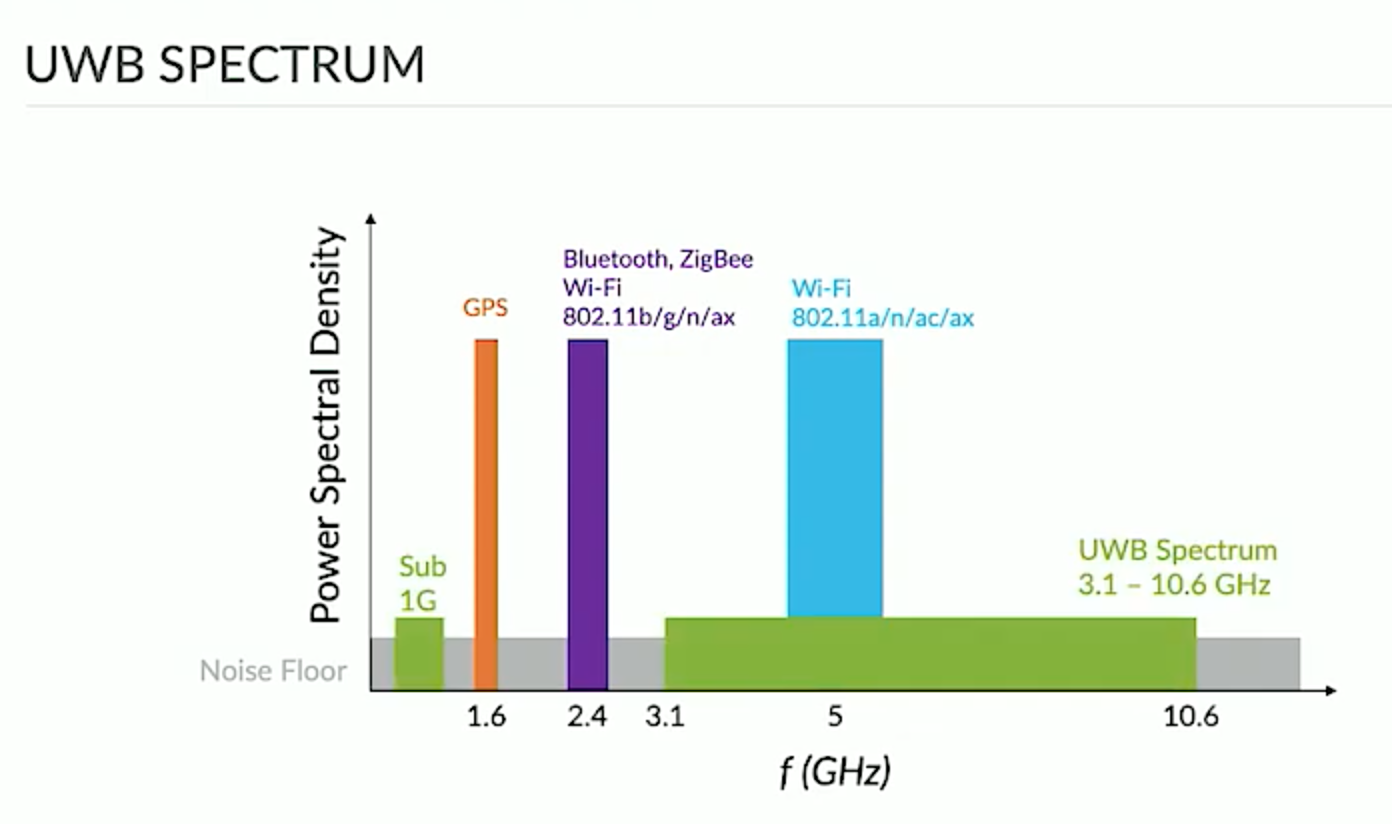
\includegraphics[width=0.8\textwidth]{./uwb_spectrum}				 
	\caption{Insufficient data.}		
	\label{img:ihuma}												 
\end{figure}

Outra característica do UBW é a utilização de rápidos pulsos (em média 2 ns entre as bordas de subida e descida) para transmitir dados, 
que são muito mais eficientes e precisos do que por alteração da frequência ou amplitude do sinal. Essa é uma das características
que fazem desta tecnologia muito útil para localização \textit{indoor}, podendo apresentar uma precisão de menos de 15 cm,
quanto outras tecnologias não chegam a 1 metro.

Uma das grandes dificuldades em localização \textit{indoor} é a perda do sinal ao ser refletido em paredes ou outros obstáculos. Considerando sinais
senoidais, a interferência entre o sinal emitido e refletido pode alterar o sinal a ponto de sua frequência e amplitude não serem
mais reconhecidas pelo receptor. Por utilizar pulsos e trabalhar numa ampla faixa de frequência, os sinais do UWB se mostram mais 
eficientes nessas situações, visto que são menos susceptíveis a estas alterações. 

Como pode ser visto na imagem acima, o UWB trabalha em uma potência significativamente mais baixa do que as outras tecnologias em 
toda sua banda, o que deixa aparelhos alimentados por baterias, como robôs móveis, muito mais eficientes, visto que gastariam menos energia
para se localizar.

\subsection{Desvantagens}
Em contrapartida às características supracitadas, UWB ainda têm sua aplicabilidade restrita por alguns fatores.
Por ser uma tecnologia ainda não muito explorada no mercado, seus equipamentos de instalação ainda são caros. Além disso,
o alcance máximo de um sinal em UWB é de, em média, 10 metros, tornando necessário o posicionamento de vários \textit{anchors} para que
o posicionamento em locais grandes se torne eficiente, o que encarece ainda mais o sistema.




%---------------picture------------------------------------
% \begin{figure}
%     \centering
%     \subfigure[Figure A]{\label{fig:a}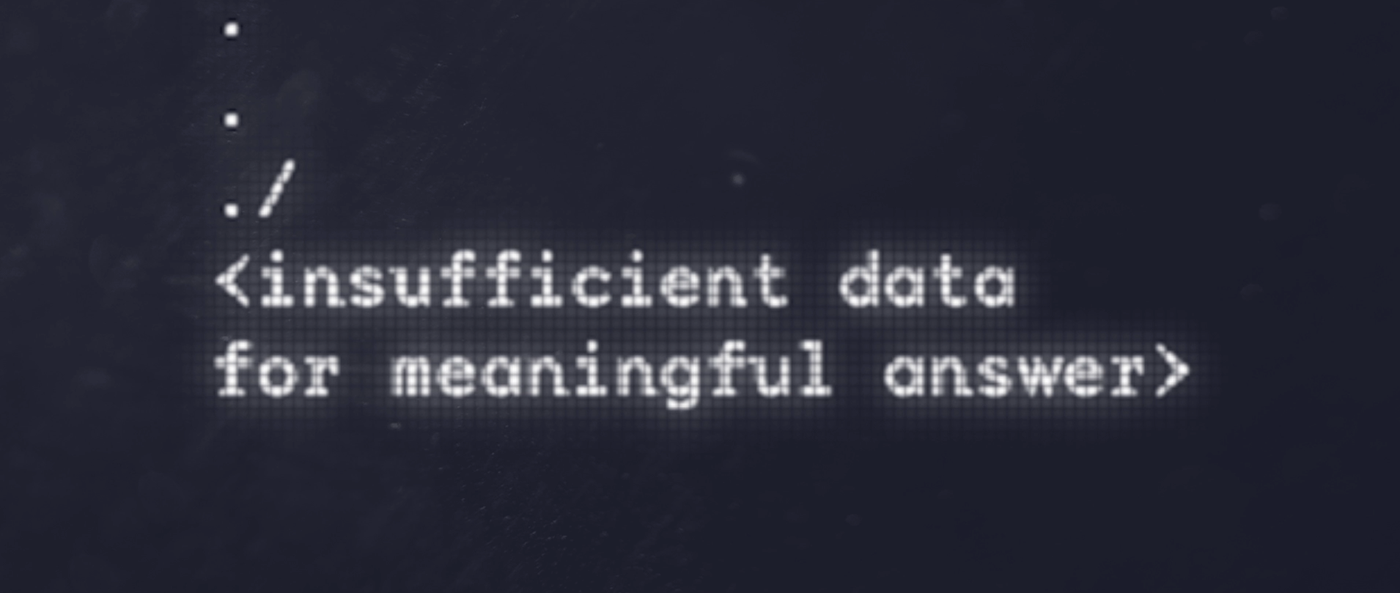
\includegraphics[width=60mm]{./lq}}
%     \subfigure[Figure B]{\label{fig:b}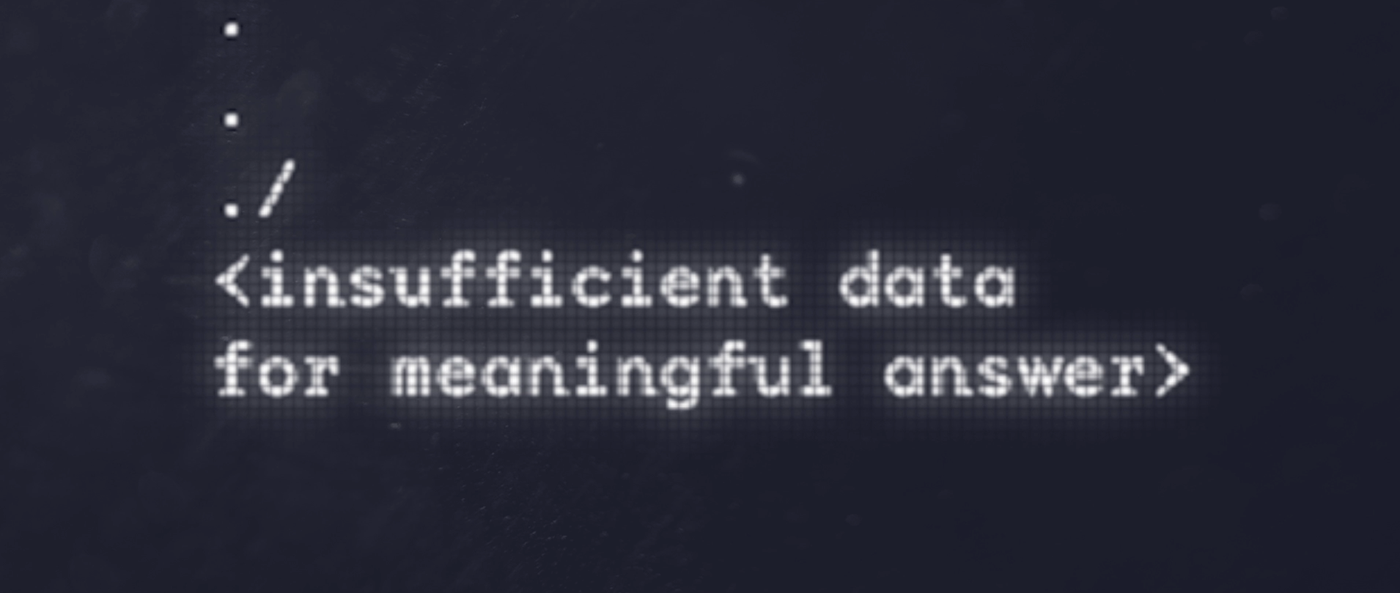
\includegraphics[width=60mm]{./lq}}
%     \subfigure[Figure C]{\label{fig:c}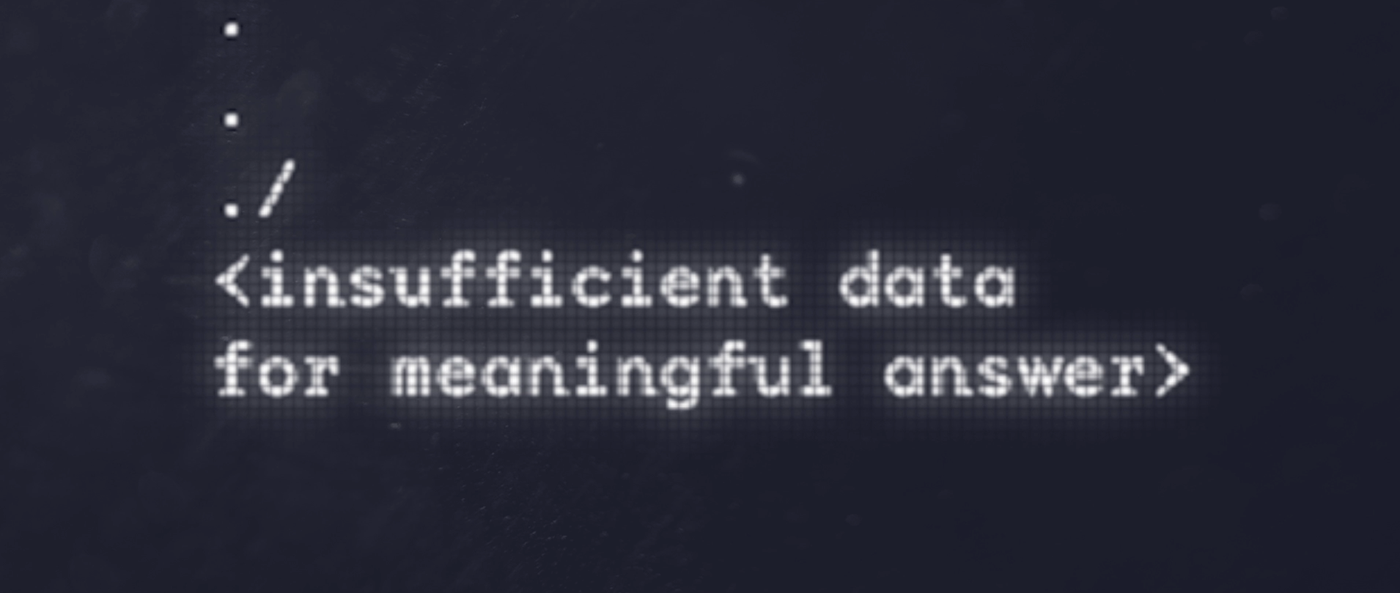
\includegraphics[width=\textwidth]{./lq}}
%     \caption{Three simple graphs}
%     \label{fig:three graphs}
% \end{figure}
%----------------------------------------------------------